Until now, authors have outlined which tasks of the linked data lifecycle can be applied to the promotion of raw data to 
linked data and they have also highlighted the main key-points in the particular case of PSCs. Thus, the selected PSCs, see Table~\ref{table:pscs-ld}, 
can be easily coded into RDF accomplishing the requirements of keeping all desired principles of this initiative. 
The selection of product scheme classifications in the e-Procurement sector has followed the next criteria: 
\begin{itemize}
 \item The use of the CPV 2008 (hereafter CVP refers to CPV 2008) is mandatory for all public procurement notices according 
 to the Regulation (EC) Nº 2195/2002 of the European Parliament and it is used as a hub classification.
 \item European classifications such as CPC or CPA have direct mappings (hand-made) to the CPV so they perfectly fit 
 to the task $t_8$ of interlinking RDF resources (\texttt{skos:exactMatch}).
 \item International classifications such as ISIC, SITC or NAICS enable the interoperability with 
 other e-Procurement and e-Commerce systems as well as activities in the field of statistics.
 \item GoodRelations and Product Ontology (PO) are two of the main references in the e-Commerce sector. 
 That is why we reuse their definitions and instances with the objective of aligning the linkage of PSCs to existing efforts. 
 \item Other classifications such as TARIC, UNSPSC, PRODCOM or NAPCS are ongoing work and they will be also linked to the CPV.
\end{itemize}

\begin{table}[!ht]
\renewcommand{\arraystretch}{1.3}
\begin{center}
\begin{tabular}[c]{|p{6cm}|l|p{6cm}|} 
\hline
  \textbf{PSC} &  \textbf{Acronym} & \textbf{Source} \\\hline
  Common Procurement Vocabulary, (2003 and 2008) & CPV & European Union \\ \hline
  Combined Nomenclature 2012 & CN & European Union \\ \hline
  Central Product Classification, version 2 (2008) & CPC & European Union \\ \hline
  Product Classification by Activity (2008) & CPA & European UnionUnión Europea \\ \hline
  International Standard Industrial Classification of All Economic Activities, Rev.4 & ISIC & \textit{United Nations Statistics Division} \\ \hline
  North American Industry Classification System 2007 y 2012 & NAICS & United States \\ \hline
  Standard International Trade Classification, Revision 4 & SITC & \textit{United Nations Statistics Division} \\ \hline
%\textit{Nomenclature générale des activités économiques dans les Communautés européennes} & NACE & Unión Europea \\ \hline
\hline
\end{tabular}
\caption{Product Scheme Classifications.}\label{table:pscs-ld}
  \end{center}
\end{table} 

Following a summary of the relevant tasks according to the MOLDEAS lifecycle is presented:
\begin{itemize}
 \item Tasks $t_1$ and $t_5$. There is an implicit structure in each product classification 
 that enables the use of graph definitions (tree and forest).
 \begin{itemize}
  \item Product categories. A PSC is divided into product categories, $Cat_{psc}$ 
  that group different elements according to hierarchy levels, these categories are disjointed sets of elements. 
  Thus, each PSC element or term is defined in only one $Cat^k_{psc}$.
  \item Taxonomy. Apart from categories and hierarchy division, each product sector can be considered as a tree, $T_{psc}$, 
  and the whole set of trees builds a forest, $F_{psc}$. Each $t^0_{psc}$  element 
  is the root of a product sector and each $t_psc$ is part of only one $T_{psc}$. According to the forest definition, 
  the set product sectors are disjointed.
 \end{itemize}

 Taking into account these points and the features of the PSC, a common model using SKOS is presented in Figure~\ref{fig:pscs-data-model}.
 
 \begin{figure}[!ht]
\centering
	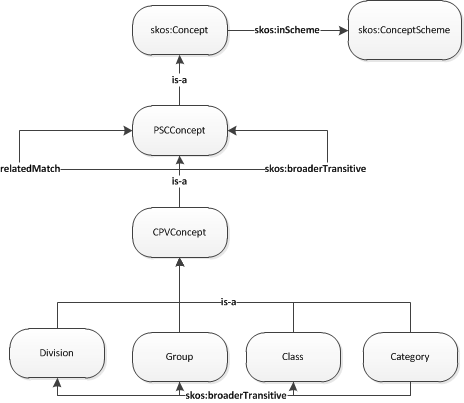
\includegraphics[width=\textwidth]{./imgs/fig-2}
 \caption{A partial view of the data model for PSCs in SKOS.}
 \label{fig:pscs-data-model}
\end{figure}

\item Task $t_6$. One of the key points to a successful promotion of raw data consists on the URI 
design~\cite{Heath_Bizer_2011}. In Table~\ref{table:pscs-uri}, PSCs URIs are presented with the aim of addressing the desired features 
of being ``Cool Uris'', meaningful, keep the namespaces under our control, etc. 
easing the reuse of RDF resources in the Web of Data.
 
 
 \begin{table}[!ht]
\renewcommand{\arraystretch}{1.3}
\begin{center}
\begin{tabular}[c]{|p{5cm}|p{4.5cm}|p{5cm}|} 
\hline
  \textbf{URI} &  \textbf{Description} & \textbf{Example} \\\hline
  \url{http://purl.org/weso/pscs/} & URI base: <base\_uri> & NA \\ \hline
  \url{<base_uri>/ontology} & Common definitions & \url{<base_uri>/ontology/PSCConcept} \\ \hline
  \url{<base_uri>/resource/ds} & Description of the PSCs Catalogue & \url{<base_uri>/resource/ds} \\ \hline
  \url{<base_uri>/{psc}/{version|year}} & PSC Namespace & \url{<base_uri>/cpv/2008} \\ \hline
  \url{<base_uri>/{psc}/{version|year}/ontology} & Specific definitions & \url{<base_uri>/cpv/2008/ontology} \\ \hline
  \url{<base_uri>/resource/{psc}/{version|year}/{id}} & URI for RDF resources & \url{<base_uri>/cpv/2008/resource/30210000} \\ \hline
  \url{<base_uri>/resource/{psc}/{version|year}/ds} & Description of the PSC dataset  & \url{<base_uri>/cpv/2008/resource/ds} \\ \hline
\hline
\end{tabular}
\caption{Design of an URI Scheme for the PSCs Catalogue.}\label{table:pscs-uri}
  \end{center}
\end{table} 

\item Task $t_8$ . The broad aim of this task is to enable the possibility of querying, 
public procurement notices from any PSC that is why there is link between any promoted PSC and the CPV. 
The mappings can be created following two approaches: 1) exact mappings created by a domain expert or 2) related, 
through the execution of a custom entity reconciliation process based on Natural Language Processing techniques, 
these mappings are automatically discovered and generated.

\end{itemize}
Once the lifecycle has been carried out the results of promoting to RDF the selected PSCs can be shown in Table , 
more specifically the first four columns specify respectively the vocabulary of a PSC ($V_{psc}$), the number of elements 
to be promoted ($V_{psc}$), the number of generated RDF triples and the number of links to the CPV. 
Thus we have promoted more than $42035$ product descriptions, generating more than $1842053$ triples and creating $21715$ 
links among them. Finally, Figure~\ref{fig:example-cpv-code}  shows an example of a generated RDF resource in which multilinguism features, 
hierarchy relationships and links can be found. Furthermore, data can be now exploited through SPARQL queries 
such as ``Give me 100 products or services related to construction in any PSC that 
have a mapping with products or services in CPV (descriptions in English)'', see Figure~\ref{fig:example-sparql-query}, using different vocabularies.

\begin{figure}[!ht]
\begin{lstlisting}[language=SQL,basicstyle=\ttfamily\footnotesize]  
cpv2008-res:30210000 a gr:ProductOrServiceModel, cpv-onto:Group;
  skos:prefLabel, gr:description, rdfs:label 	
  "Tietojenkäsittelylaitteet (laitteisto)"@FI ,
  "Andmetöötlusmasinad (riistvara)"@ET , 
  "Μηχανές επεξεργασίας δεδομένων (υλισμικό)"@EL , 
  "Datenverarbeitungsgeräte (Hardware)"@DE , 
  "Stroje na zpracování dat (technické vybavení)"@CS ,
  "Magni għall-ipproċessar tad-dejta (ħardwer)"@MT , 
  "M\'{a}quinas de processamento de dados (hardware)"@PT , 
  "Machines de traitement des données (matériel)"@FR ,
  "Duomenų apdorojimo mašinos (techninė įranga)"@LT , 
  "Naprave za obdelavo podatkov (strojna oprema)"@SL , 
  "Databehandlingsmaskiner (hardware)"@DA ,
  "Macchine per l'elaborazione di dati (hardware)"@IT ,
  "Stroje na spracovanie údajov (hardvér)"@SK , 
  "Databehandlingsmaskiner (maskinvara)"@SV ,
  "Adatfeldolgozó gépek (hardver)"@HU ,
  "Maşini de procesare a datelor (hardware)"@RO , 
  "Data-processing machines (hardware)"@GA ,
  "Data-processing machines (hardware)"@EN ,
  "Maszyny do przetwarzania danych (sprzęt)"@PL , 
  "Машини за обработване на данни (хардуер)"@BG ,
  "Machines voor dataprocessing (hardware)"@NL , 
  "Datu apstrādes iekārtas (aparatūra)"@LV ,
  "M\'{a}quinas procesadoras de datos (hardware)"@ES ;
  dct:identifier "30210000"^^xsd:string;
  dct:subject "30210000-4"^^xsd:string;
  pscs-onto:relatedMatch   
    <http://www.productontology.org/id/dataprocessing>,
    <http://www.productontology.org/id/hardware> ,
    <http://www.productontology.org/id/machine> ;	
  skos:broaderTransitive cpv2008-res: 30200000;
  skos:exactMatch 
    cpv2003-res:30216000, cpv2003-res:30215000,  cpv2003-res:30213000,   
    cpv2003-res:30212000, cpv2003-res: 30211000,  cpv2003-res:30214000.
\end{lstlisting}
\caption{Example of CPV 2008 item in RDF.}
 \label{fig:example-cpv-code}
\end{figure}


\begin{figure}[!ht]
\begin{lstlisting}[language=SQL,basicstyle=\ttfamily\footnotesize]  
SELECT DISTINCT * WHERE{
   ?product pscs:relatedMatch 
    <http://www.productontology.org/id/construction> .
   ?product skos:closeMatch ?cpv .
   ?product skos:prefLabel ?productLabel .
   ?cpv skos:prefLabel ?cpvLabel .
   ?product skos:inScheme ?scheme .
   FILTER (?scheme != <http://purl.org/weso/pscs/cpv/2008/resource/ds>) .
   FILTER (lang (?cpvLabel) ="en " )
} LIMIT 100
\end{lstlisting}
\caption{Example of SPARQL query.}
 \label{fig:example-sparql-query}
\end{figure}

